% $Id$

One of the most interesting problems in astrophysics is that of \emph{dark
matter}. Dark matter is material in the universe that interacts
gravitationally with luminous matter, but has so far eluded direct
observation. 


There have been several  the nature of dark matter,
chief among these are WIMPs and MACHOs. WIMPs are \emph{weakly interacting
massive particles}, supersymmertic particles produced as a relic of the big
bang, and are outside the scope of this thesis\footnote{We refer to
\cite{Griest:1995gs} for a review of the nature of dark matter.}. Here we are
concerned with the proposeal that a component of the dark matter is in the
form of \emph{massive astrophysical compact halo objects} or
MACHOs\cite{Griest:1990vu}. Possible candidates for MACHOs are brown dwarfs,
Jupiters or black hole remnants from an early population of stars.

of WIMPs or MACHOs (or some combination of the two).  WIMPs, , are outside the scope of this
thesis
In this chapter, we review the evidence for a form of dark matter
known as massive astrophysical compact halo objects (MACHOs)\cite{x}


Dark matter is so called because it has eluded detection through its
emission or absorbsion of electomagnetic radiation. Our knowlege of its
existance comes from the gravitational interaction of dark matter with
luminous matter in the universe. There are two major theories proposed to
explain the origin of dark matter. The first is that they are weakly
interacting massive particles (WIMPs). WIMPs are a concequency of
supersymmertry and are outside the scope of this thesis; we refer the
interested reader to \cite{XXX}.  In this thesis, we are concered with the
proposal that a some component of the dark matter consists of massive
astrophysical compact halo objects (MACHOs), in particular the possibility
that MACHOs may be primordial black holes (PBHs) formed in the early universe.
In this chapter, we review the evidence for dark matter in the universe and
describe how it may be possible to detect a proposed population of PBHs in the
galactic halo.

\section{Dark Matter In The Galactic Halo}
\label{s:darkmatter}

Dark matter is detected by its gravitational interaction with luminous matter.
Strong evidence for the presence of dark matter in the universe comes from the
study of galactic rotation curves; measurements of the velocities of luminous
matter in the disks of spiral galaxies as a function of galactic radius.  Let
us consider a simple rotational model for the disk of a spiral galaxy.
Consider a star with mass $m_s$ orbiting at radius $r$ in the outer part of
the galaxy's disk. Newtonian dynanics tells us that if the mass inside radius
$r$ is $m_g$ then
\begin{equation}
\frac{Gm_g m_s}{r^2} = \frac{m_s v_s^2}{r}
\label{eq:newtongalaxy}
\end{equation}
where $v_s$ is the velocity of the star and $G$ is the gravitational constant. 
If we assume that as we increse $r$, the change in the $m_g$ is negligable.
This is a reasonable assumption towards the edge of the disk, since the mass
is concentrated towards the center of the galaxy.  We can see from equation
\ref{eq:newtongalaxy} that we would expect that the velocity of stars at the
edge of the galactic disk would fall off as 
\begin{equation}
v_s \propto \frac{1}{\sqrt{r}}
\end{equation}
and so a typical galactic rotation curve would fall off as $r^{-1/2}$.
Galactic rotation curves, measuring using the doppler shift of the
$21$~cm hydrogen line, have been measured for several galaxies. It is found
that the rotation curves to not fall off as expected. Instead they are flat
out to the edge of the visible matter in the disk, as shown in
figure~\ref{f:rotcurves}.  This surprising result suggests that most of the
matter in galaxies does not emit light but is gravitationally coupled to the
visible matter. Rotation curves suggest that around 80\%--90\% of the matter
in spiral galaxies is in the form of dark matter\cite{Sancisi:1987}.

Since we have been unable to observe the dark matter component of the galaxy,
we must infer its distribution and density from the indirect obesrvations and
numerical simulations of galaxy formation. Consider the evolution of a spatial
distribution of baryonic matter. Baryonic matter is the typical luminous
matter that we see composed of neutrons, protons, electrons and other baryons.
If the distribution is initially spherical and rotating with some angular
momentum, $L$, then over time the matter will lose energy through inelastic
collisions. Since the angular momentum of the system must be conserved,
howeverm the initial distribution will collapse to a rotating disk.  This toy
model is typical of the formation of galaxtic disks from baryonic matter. On
the other hand, if the initially spherical distribution is composed of dark
matter, the only collisions that the population will undergo are elastic,
because the dark matter is weakly interacting. As a result of this, if the
dark matter is initially distributed uniformly with and isotropic, it will
maintain this distribution as it evolves.

We may guess that the dark matter halos are at least as old os the visible
matter as they are much more massive. Since the dark matter is gravitationally
bound to the visible matter in the disk, it is reasonable to assume that the
visible disk and dark halo are in thermal equilibrium with some characteristic
mean square velocity. Since we do not expect a spherical dark matter halo to
collapse to a disk, the simplest possible assumption is that the dark halo is
a spherical, isothermal distribution of dark matter. We may ask what the
dark matter density is in the neighbourhood of the earth. If we assume that
the density of the dark matter is $\rho(r)$ then for a spherical halo the mass
within a thin shell of width $dr$ is
\begin{equation}
dM(r) = 4\pi r^2 \rho(r)\, dr.
\label{eq:simplehalodensity}
\end{equation}
Using Newtonian dynamics, the velocity, $v$, of a particle of mass $m$ at
radius $r$ is
\begin{equation}
\begin{split}
\frac{GM(r)m}{r^2} &= \frac{mv^2}{r} \\
v^2 &= \frac{GM(r)}{r}.
\end{split}
\end{equation}
The galactic rotation curves tell us that the velocity is independent of the
radius, so
\begin{equation}
M(r) = \frac{v^2r}{G}.
\end{equation}
Differentiating this with respect to $r$ and substituting the result into
equation \ref{eq:simplehalodensity}, we obtain
\begin{equation}
\frac{dM(r)}{dr} = \frac{v^2}{G} = 4\pi r^2\rho(r)
\end{equation}
which gives
\begin{equation}
\rho(r) = \frac{v^2}{4\pi r^2 G}.
\label{eq:simplehalodensity2}
\end{equation}
Since the dark and visible matter are in thermal equilibrium, we may use the
measrued rotational velocity of local stars about the galactic center as the
velocity of the dark matter. The earth is approximately $8$~kPc from the
galactic center and the rotational velocity of objects at this radius is
$v\sim 200\mathrm{km\,s}^-1$. Using these values in equation
(\ref{eq:simplehalodensity2}), we obtain a value of
\begin{equation}
\rho(r_E) = 7.6 \times 10^{-25}\, \mathrm{g}\,\mathrm{cm}^{-3}.
\end{equation}
Clearly equation (\ref{eq:simplehalodensity2}) cannot be true at all radii, as
it suggests that $\rho \rightarrow \infty$ as $r \rightarrow \infty$. It is
observered that rotation velocities fall to zero as $r\rightarrow 0$. The data
at small $r$ is consistent with the dark matter having a constant \emph{core
density}, $\rho_c$ within a \emph{core radius}, $a$. The halo density then
becomes
\begin{equation}
\rho(r) = \frac{\rho_c}{1 + \left(\frac{r}{a}\right)^2}.
\label{eq:simplehalodensity3}
\end{equation}.
The values of $\rho_c$ and $a$ are obtained from fitting measured galactic
rotation curves to equation (\ref{eq:simplehalodensity3}) using data near the
galactic center. 

There is, in fact, no evidence to suggest that halos are
exactly spherical; the halo density may be flattened\cite{Rix:1996}. For a
flattened halo the dark matter density becomes
\begin{equation}
\rho(R,z) = \frac{\rho_c r^2_c}{a^2 + R^2 + z^2/q^2}
\label{eq:simplehalodensity4}
\end{equation}
where $R$ and $z$ are galactocentric cylindrical coordinates and $q$ is a
parameter that describes the flattening of the halo. Careful modelling of the
Galaxy\cite{1995ApJ...449L.123G}, suggests that the local halo density is
\begin{equation}
\rho_(r_E) = 9.2_{-3.1}^{+3.8} \times 10^{-25}\,  \mathrm{g}\,\mathrm{cm}^{-3}
\end{equation}
or approximately $0.01\,M_\odot.\,\mathrm{pc}^{-3}$.

\section{Gravitational Microlensing}
\label{s:microlensing}


\section{Gravitational Waves from Binary Black Hole MACHOs}
\label{s:bbhmacho}

Since the microlensing surveys have shown that some $\sim 20\%$ of the halo
dark matter is in the form of $\sim 0.5\,M_\odot$ MACHOs, it is natural to ask
what the nature of these MACHOs are. MACHOs could be baryonic matter in the
form of brown dwarfs, objects lighter than $\sim 0.1\,M_\odot$ that do not
have sufficient mass to sustain fustion. Brown dwarfs are to light to be
candiates for MACHOs, however. Observations of red dwarfs, the faintest
hydrogen burning stars with masses greater than $\sim 0.1\,M_\odot$, using
Hubble Space Telescope data constrain both the fraction of halo in red and
brown dwarfs. It is found that brown dwarfs make up less than $\sim 3\%$ and
red dwarfs less than $\sim 1\%$ of the halo \cite{Graff:1995ru,Graff:1996rz}.
A third possible candidate for baryonic MACHOs is a population of ancient
white dwarfs in the halo. White dwarfs have masses of $\sim 0.6\,M_\odot$ and
so seem to be natural candidates for MACHOs. They are the remnants of stars of
mass $1$--$8\,M_\odot$. Searches for halo white dwarfs have been conducted and
no candidates have 
found\cite{2002A&A...389L..69G,2002ApJ...573..644N,Creze:2004gs}. The latest
results, which combining results from these three surveys, suggest that less
that $4\%$ ($95\%$ confidence level) of the halo is in the form of white
dwarfs\cite{Creze:2004gs}. 

It is possible that there is an overdense clump of MACHOs in the direction of
the LMC\cite{1996ApJ...473L..99N}, the lenses are located in the LMC
itself\cite{Salati:1999gd} or in the disk of the galaxy\cite{Evans:1997hq}. 
If the MACHOs detected by microlensing are truely in the halo, however, it is
possible that MACHOs are non-baryonic matter such as black holes
\cite{Nakamura:1997sm}. Black holes of mass $\sim 0.5\,M_\odot$ could not have
formed as a product of stellar evolution and so they must have been formed in
the early universe\cite{1971MNRAS.152...75H,1974MNRAS.168..399C}. 

\section{BBHMACHO Population Model}
\label{s:bbhmachopopulation}

The goal of this thesis is to search for the gravitational waves from binary
black hole MACHOs described in the previous section. In the absence of a
detection, however, we wish to place an \emph{upper limit} on the rate of
BBHMACHO inspirals in the galaxy. We can then compare the predicted rate
with that determined by experiment. We will see later that in order to
determine an upper limit on the rate, we need to mesure the \emph{effiency},
$\epsilon$, of our search to BBHMACHOs in the galactic halo. We do this
using a Monte Carlo simulation which generates a population of BBHMACHOs from
a given probability density function of the BBHMACHO parameters. Using the
set of parameters generated by sampling the PDF, we can simulate the inspiral
waveforms on a computer. We then digitally add the simulated waveforms to the
output of the gravitational wave detector after the data has been recorded to
disk. This process is refered to as \emph{software injection}. By analyzing
the interferometer data containing the injected signals we can determine how
many events from the known source distribution we find. The efficency of the
search is then simply
\begin{equation}
\epsilon = 
\frac{\textrm{number of signals found}}{\textrm{number of signals injected}}.
\end{equation}
Recall that an inspiral waveform is described by the following nine 
parameters:
\begin{equation*}
\begin{split}
t_c &\quad \textrm{the end time of the inspiral}, \\
m_1 &\quad \textrm{the mass of the first binary component}, \\
m_2 &\quad \textrm{the mass of the second binary component}, \\
\iota &\quad \textrm{the inclination angle of the binary}, \\
\phi_c &\quad \textrm{the coalescence phase of the binary}, \\
\psi &\quad \textrm{the polarization angle of the binary}, \\
(R,\theta,z) &\quad \textrm{the galactocentric cylindirical coordinates of the
binary}.\\
\end{split}
\end{equation*}
In this section describe how a simulated population of galactic BBHMACHOs is
generated by sampling the probability density functions of these parameters.

We first address the generation of inspiral end time, $t_c$. The nature of the
noise in the interferometers changes over the course of the run, as does the
orientation of the detectors as the earth rotates about its axis over a
siderial day. To sample the changing nature of the detector output, the Monte
Carlo population that we generate contains many inspiral signals with end
times distributed over the course of the science run. We generate values of
$t_c$ at fixed intervals starting from a specifted time $t_0$. The fixed
interval is typically chosen to be $2630/\pi \approx 837.155000663$~sec. This
allows us to inject a significant number of signals over the course of the two
month run with the signals are far enough appart that they will not dominate
the power spectrum of the detector output. The interval is chosen to be a
non-integer so to avoid any possible periodic behavour in the detector output.
The start time for the Monte Carlo, $t_0$, is chosen from a uniform random
distribution in the range $t_\mathrm{S2} - 2630/\pi \le t_0 \le
t_\mathrm{start}$, where $t_\mathrm{start}$ is the time at which the science
run begins. We stop generating inspiral parameters when $t_c > t_\mathrm{end}$
the time at which the second science run ends. For each generated end time,
$t_c$ we generate then generate the other eight inspiral waveform parameters.

We obtain the distribution of the mass parameters $(m_1,m_2)$ from the
microlensing observations of MACHOs in the galactic halo, decribed in section
\ref{s:microlensing}. These suggest that the most likely MACHO mass is between
$0.15$ and $0.9\,M_\odot$. The absence of further information on the mass
distribution suggests that we simply generate each component mass from a
uniform distribution in this range. We will see in chapter \ref{ch:pipeline},
however, that searching for BBHMACHOs of mass lower than $0.2\,M_\odot$ is
prohibited by the amount of computational resources required. We also note
that the search for binary neutron stars covers the mass range $1$ to
$3\,M_\odot$, so we continue the BBHMACHO search up to $1\,M_\odot$ rather
than terminating it at $0.9\,M_\odot$. We therefore generate each BBHMACHO
mass parameter, $m_1$ or $m_2$, from a uniform distribution of masses between
$0.2$ and $1.0\,M_\odot$.

The angles $\iota$ and  $\psi$ are generated randomly to reflect a
uniform distribution in solid angle; $\cos \iota$ is uniform between $-1$ and
$1$ $\psi$ are uniform between $0$ and $2\pi$. The coalescence phase $\phi_c$
is also generated from a uniform distribution between $0$ and $2\pi$.

To generate the spatial distribution of BBHMACHOs, we assume that the
distribution in galactocentric cylindrical coordinates, $(R,\theta,z)$,
follows the halo density given by equation (\ref{eq:simplehalodensity4}),
that is,
\begin{equation}
\rho(r) \propto \frac{1}{a^2 + R^2 + z^2/q^2}
\end{equation}
where $a$ is the halo core radius and $q$ is the halo flatening parameter. We
can see that this distibution is independent of the angle $\theta$, so we
generate $\theta$ from a uniform distibution between $0$ and $2\pi$.  If
we make the coordinate change $z/q \rightarrow z$, then we may obtain a
probability density function (PDF) for the spatial distribuation of
the MACHOs given by
\begin{equation}
f(R,z)\,R\, dR\, dz \propto \frac{1}{a^2 + R^2 + z^2}\,R\, dR\, dz.
\label{eq:spacepdf}
\end{equation}
We wish to randomly sample this PDF to obtain the spatial distribution of
the BBHMACHOs. Once we have obtained a value of the new coordinate $z$, we
simply scale by $q$ to obtain the original value of $z$. Recall that for a
probability density function, $f(x)$, the cumulative distribution, $F(X)$,
given by
\begin{equation}
F(X) = \int_{-\infty}^X f(x)\, dx
\end{equation}
is uniformly distibuted over the interval $[0,1]$ for all $f(x)$. Hence a
random variable, $u$, uniformly distributed between $0$ and $1$ can be
interpreted as a random sample of $F(X)$. If we generate a value of $u$, we
can solve 
\begin{equation}
\int_{-\infty}^x f(x')\, dx' = u
\label{eq:goldenrule}
\end{equation}
to obtain the value of $x$. Notice, however, that PDF in equation
(\ref{eq:spacepdf}) is a function of the two random variables $R$ and $z$,
rather than a single variable, $x$, as in equation (\ref{eq:goldenrule}).
Let us make the coordinate change
\begin{equation}
\begin{split}
R &= r \cos \varphi \\
z &= r \sin \varphi \\
\label{eq:probcoordtrans}
\end{split}
\end{equation}
and so
\begin{equation}
\begin{split}
\tan \varphi &= \frac{z}{R} \\
r^2 &= R^2 + z^2 \\
\end{split}
\end{equation}
Equation (\ref{eq:spacepdf}) becomes
\begin{equation}
\begin{split}
\mathcal{K} \int_0^{R_\mathrm{max}}\int_{-\infty}^{\infty} \frac{1}{a^2 + R^2 + z^2}\,R\, dR\, dz 
&= \mathcal{K} \int_0^{R_{\mathrm{max}}}\int_{-\frac{\pi}{2}}^{\frac{\pi}{2}} \frac{r\cos\varphi}{a^2+r^2}\,r\, dr \, d\varphi \\
&= \mathcal{K} \int_{-1}^{1} d\sin\varphi \int_0^{R_{\mathrm{max}}} \frac{r^2}{a^2+r^2}\, dr \\
&= \mathcal{K} \left[\sin\varphi\right]_{-1}^1 \left[r -
a\arctan\left(\frac{r}{a}\right)\right]_0^{R_{\mathrm{max}}}
\end{split}
\label{eq:bothpdfs}
\end{equation}
where $\mathcal{K}$ is a constant that normalizes the PDF to unity. We can see
immediately from equation (\ref{eq:bothpdfs}) that $\sin\varphi$ is uniformly
distributed between $-1$ and $1$. Now consider the PDF for $r$ given by
\begin{equation}
f(r) = \mathcal{K} \left[r - a\arctan\left(\frac{r}{a}\right)\right]_0^{R_{\mathrm{max}}}
\end{equation}
In order that this is correctly normalized, we must have
\begin{equation}
\mathcal{K} = 
\left[R_\mathrm{max} -
a\arctan\left(\frac{R_\mathrm{max}}{a}\right)\right]^{-1}
\end{equation}
and so to sample the distribution for $r$ we generate a random variable, $u$,
uniform between $0$ and $1$ and find the root of
\begin{equation}
r - a\arctan\left(\frac{r}{a}\right) - u \left[R_\mathrm{max} -
a\arctan\left(\frac{R_\mathrm{max}}{a}\right)\right] = 0.
\label{eq:rroot}
\end{equation}
We can see that the value of $r$ that solves equation (\ref{eq:rroot}) must
lie between $0$ and $R_\mathrm{max}$ and that the left hand side is a
monotonically increasing function of $r$. We may therefore use a simple 
bisection to solve for the value of $r$. Once we have obtained values of $r$
and $\varphi$ we may obtain the values of $R$ and $z$ using equation
(\ref{eq:probcoordtrans}). 

We have now demonstrated how to simulate the nine pararameters of the BBHMACHO
injections. The software used to perform an injection Monte Carlo generates a
population of inspiral signals described by their end times, $t_c$. For each
$t_c$ we then generate the other 8 parameters of the inspiral as described
above. Figure \ref{f:m1_hist} shows a histogram of the first mass parameter 
generated the paremeter Monte Carlo code. It can be seen that this is uniform
between $0.2$ and $1.0\,M_\odot$, as expected. Figures
\ref{f:spherical_cartesian} shows the spatial distribution of BBHMACHO
binaries for a speherical, $q=0$, halo that extends to $R_\mathrm{max} =
50\,\mathrm{kpc}$ with a core radius of $a = 8.5\,\mathrm{kpc}$, typical
values for the Milky Way. Since the sotfware that simulates inspiral waveforms
expects the position of the inspiral to be specified in equatorial
coordinates, the population Monte Carlo code also generates the coordinates of
the inspiral as longitude, latitude and distance from the center of the
earth, as shown in figure \ref{f:spherical_equatorial}.  We will return to the
use of population Monte Carlos in chapter \ref{ch:result}.

\newpage

\begin{figure}[p]
\begin{center}
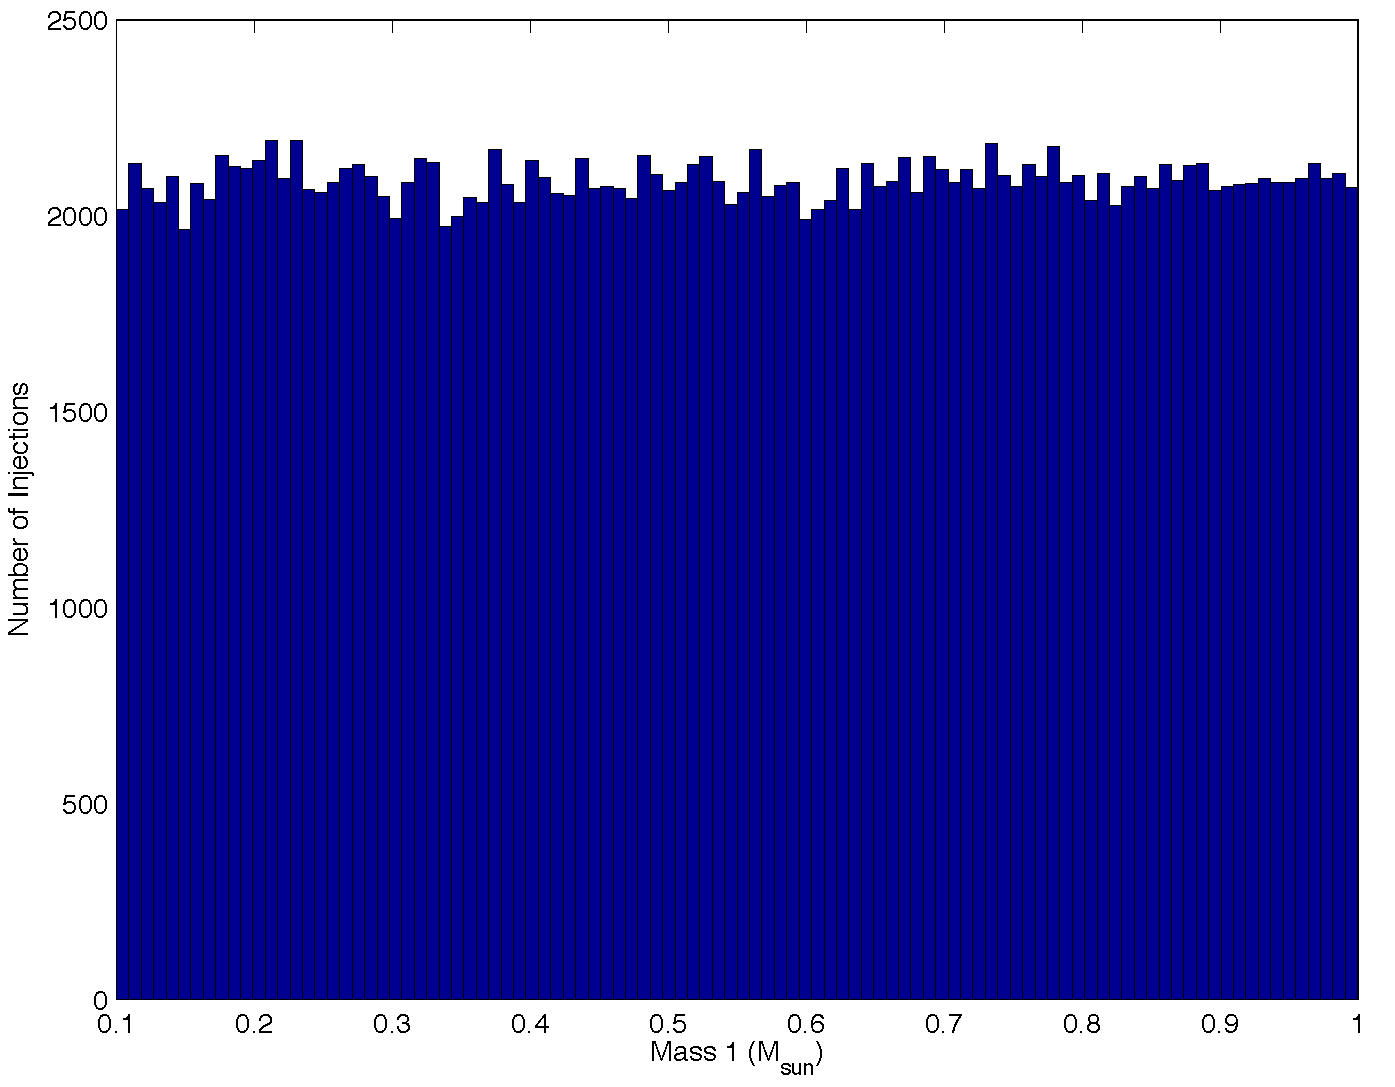
\includegraphics[width=\linewidth]{figures/macho/m1_hist}
\end{center}
\caption{\label{f:m1_hist}%
The BBHMACHO population Monte Carlo code is used to simulate a distribution of
$209048$ coalescing binaries. The distribution of the first component mass,
$m_1$ is then histogramed to confirm that it is uniformly distributed over the
expected range, as shown. Similar tests are performed for the second mass
parameter, $m_2$, the galactocentic longitude, $\theta$, the inclination
angle, $\iota$, the polarization angle, $\psi$, and the coalescence phase,
$\phi_c$.
}
\end{figure}

\begin{figure}[p]
\begin{center}
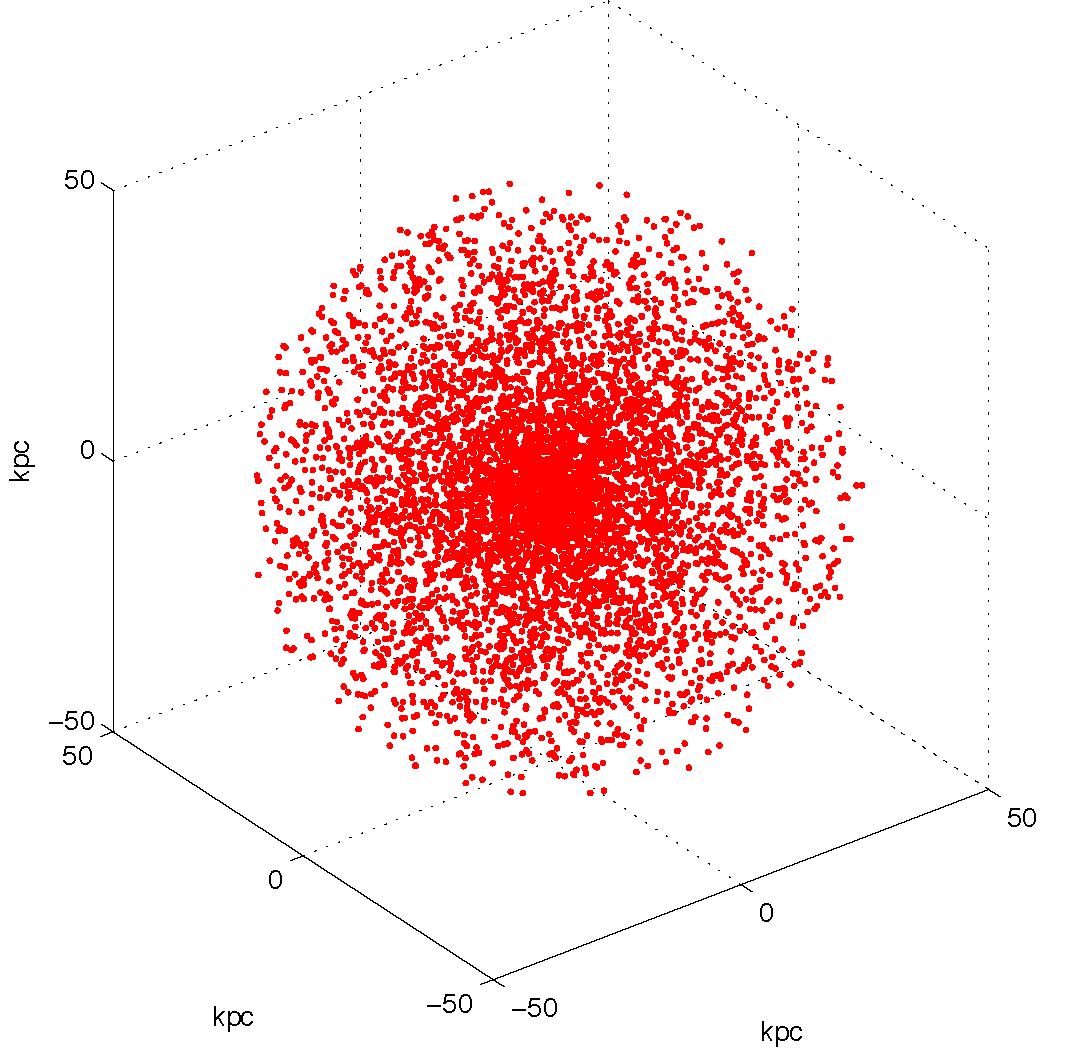
\includegraphics[width=\linewidth]{figures/macho/spherical_cartesian}
\end{center}
\caption{\label{f:spherical_cartesian}%
The spatial distribution of $5000$ simulated BBHMACHO binaries in a spherical,
$q=0$, Galactic halo of size $R_\mathrm{max} = 50\,\mathrm{kpc}$ with a core
radius $a = 8.5\,\mathrm{kpc}$ shown in galactocentric coordinates. Each point
in the figure corresponds to a simulated BBHMACHO injection.
}
\end{figure}

\begin{figure}[p]
\begin{center}
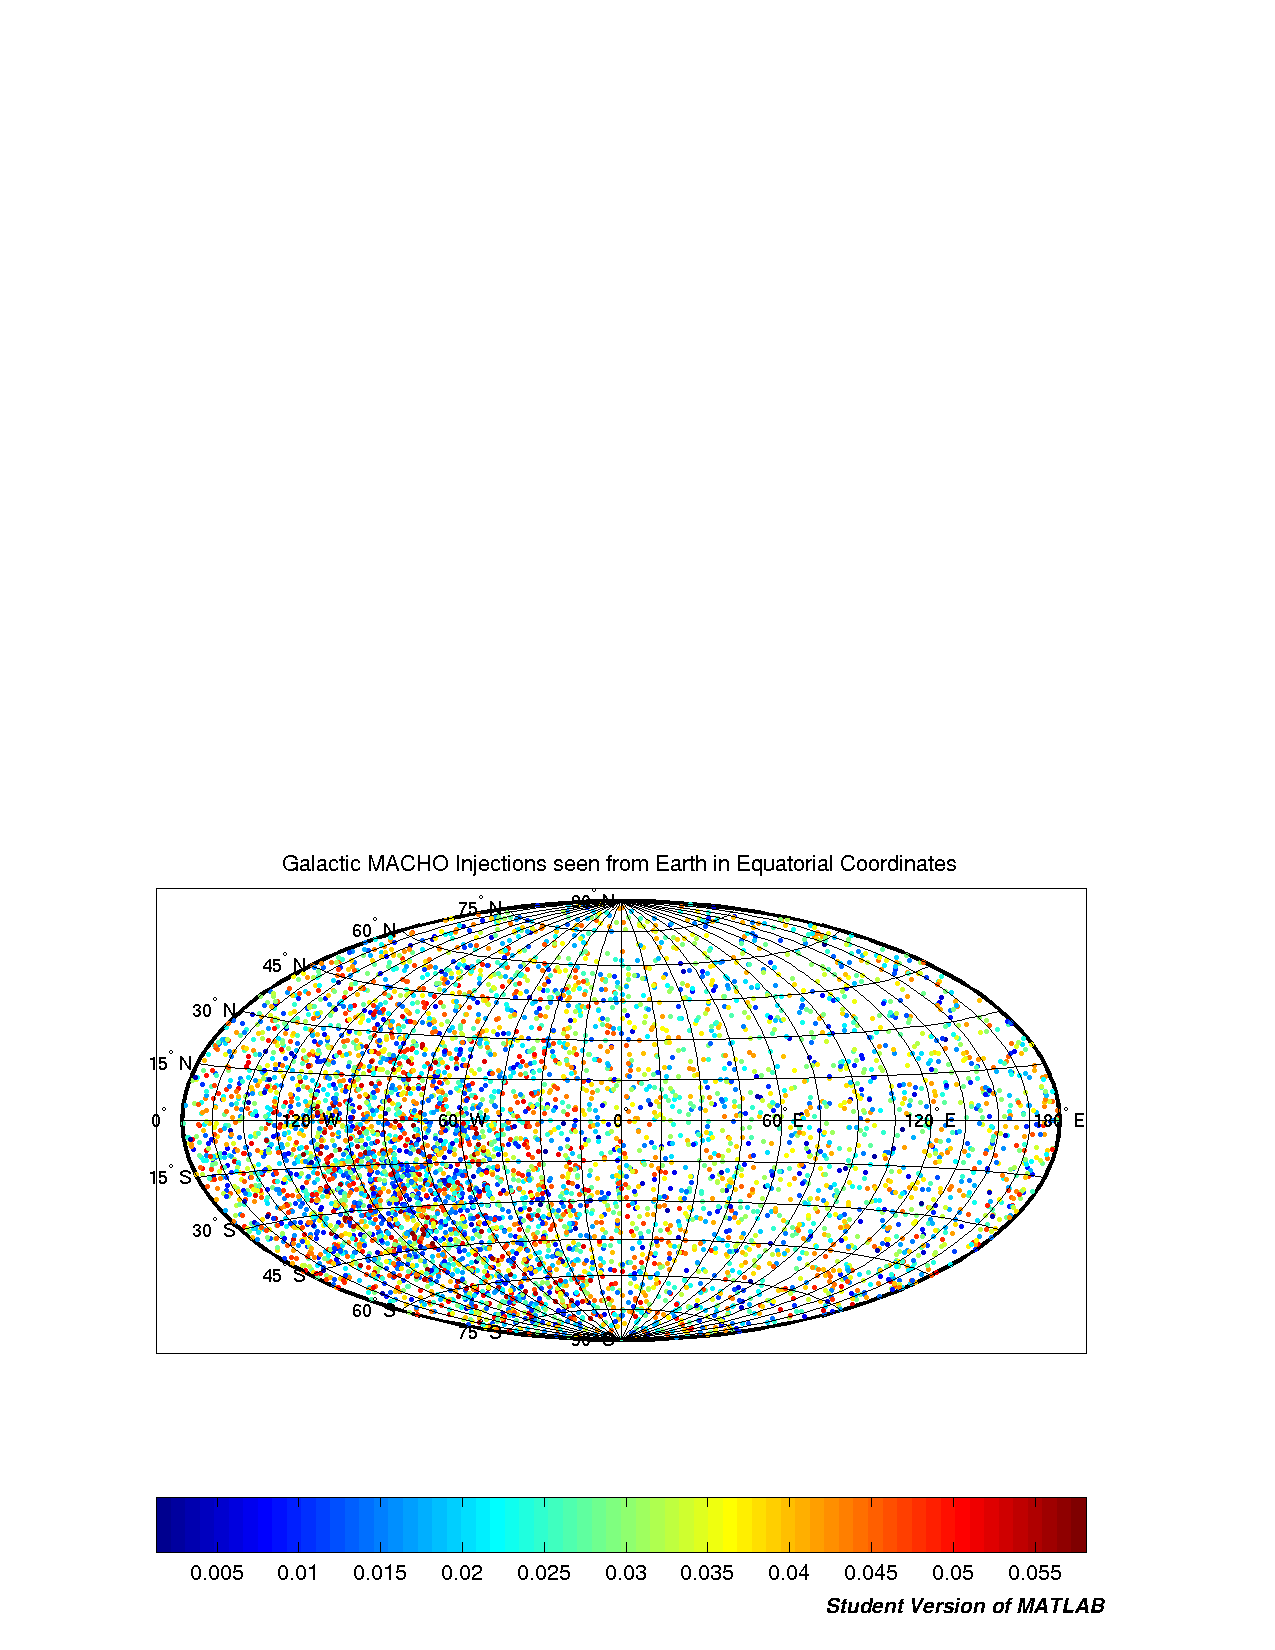
\includegraphics[width=\linewidth]{figures/macho/spherical_equatorial}
\end{center}
\caption{\label{f:spherical_equatorial}%
The spatial distribution of $5000$ simulated BBHMACHO binaries in a spherical,
$q=0$, Galactic halo of size $R_\mathrm{max} = 50\,\mathrm{kpc}$ with a core
radius $a = 8.5\,\mathrm{kpc}$ shown in equatorial coordinates. Each point
in the figure corresponds to a simulated BBHMACHO injection. The color of the
point shows the distance from the center of the earth to the binary. Note the
dense clump of binaries in the southern hemisphere, towards the center of the
galaxy.
}
\end{figure}




